\documentclass{article}
\usepackage[utf8]{inputenc}
\usepackage{amsmath}
\usepackage{amssymb}
\usepackage{parskip}
\usepackage{graphicx}
\graphicspath{ {./samples/midterm/} }
\usepackage{biblatex}
\addbibresource{midterm-references.bib}

\newcommand*{\Pn}[1]{\left( #1 \right)}

\DeclareMathOperator{\Tr}{Tr}

\title{Matrix Bubbling}
\author{Adam Busis, Jacky Lee, Princewill Okoroafor}
\date{November 2, 2018}

\begin{document}

\maketitle

\section{Abstract}

Matrix bubbling is a useful technique for analyzing big data sets because it
collapses the large amount of data given into a smaller matrix of summary
statistics, which is easier to work with. In this paper, we discuss matrix
bubbling in two dimensions but this technique can be easier extended to
higher-dimensional space.

\section{Background}

When working with big data, it often takes a long time to process data since
there is so much of it. To try to resolve this problem, we want to be able to
somehow reduce this data into its essence such that we numerically have less
data to work with, which means we can process it faster, but still have
sufficient information to extract something meaningful out of it.\\

One method that does this is called dimension reduction. The general idea of
dimension reduction is that we can reduce the number of variables involved in
our data such that we have less to work with but still enough information to
perform computations with. Dimension reduction is a useful tool that enables us
to analyze big data sets with less computation time.\\

Generally, this is done by determining which features define the data the most
and restricting our attention to those few features. For example, consider the
scenario where we want to read characters off of hand-drawn maps. Given a
random symbol from the map, how do we determine whether the symbol is a letter
or just some junk from the map? There can be a lot of information hidden within
each symbol. One thing we could do is to only consider specific features that
seem to be the most important for determining whether a symbol is a letter or
not. For example, we can only look at the width, height, and density of the
input and from there guess whether the symbol is a letter or not. This is
plausible because letters on a map generally are within some size limit; they
are probably not too big (taking up a quarter of the map) and they are probably
not too small (taking up just 3 pixels worth of space).\\

Another thing that can be done is to define new features that can be thought of
as combinations of multiple features. For example, we could replace our width
and height feature for a new perimeter feature, which is computed by taking the
sum of the width and height then multiplying by 2. We see that this perimeter
feature is a combination of both the width and height features.\\

Currently, the main dimension reduction technique is called Principle Component
Analysis, or PCA for short. Essentially, this method takes in data and computes
the most important features that help identify the data.

\section{Motivation}

Let us restrict our attention to the two-dimensional case for now since it is
easier to visualize. Suppose we have a large set of data distributed in
two-dimensional space in a fashion that is not Gaussian. For example, the
pixels representing the letter `A' are not distributed normally. Now suppose we
would like to compare it with another data set that is also large and
distributed in some space. Let's call these two data sets $A$ and $B$. One way
to do it is to take each data point's location in the space and compare it to
the analogous space in the other data set. This requires going through each
point and requires a lot of computations.\\

The idea behind matrix bubbling is that we can somehow summarize each data set
using some proxy such that if we want to compare two data sets $A$ and $B$, we
can simply compare their proxies, $A_p$ and $B_p$, where the proxies are much
smaller than the original data sets. The ``proxy'' can be any smaller set of
data depending on the data set. This can be thought of as a sort of dimension
reduction since we are reducing the amount of data we need to consider and
instead summarizing the data using a few key statistics. Ideally, the proxies
for two different data sets will be close together if (and only if) the two
data sets are similar, where similarity of the data sets is a criterion that
depends on the application.\\

One possible way of summarizing the data would be to look at summary statistics
for the entire data set, such as the mean and variance. The problem with this
method is that just the mean and variance for the entire data set don't have
enough information to capture the nuances of the data set. The key idea is that
we can view our space as a grid and partition this grid into smaller grids.
Then for each grid, we can find a probability distribution that summarizes the
data within that grid and use it as a proxy. Since probability distributions
can be summarized by a few statistics such as the mean and covariance for a
Gaussian distribution, this reduces the number of data points we have to
consider. By changing the number of smaller grids (and therefore the size of
the smaller grids) that we divide the data set into, we can adjust the fineness
of the details we look at in the data based on the application.

\section{Introduction}

Suppose we have a matrix $M$ representing a two-dimensional data set which we
would like to compare to another matrix $N$ representing a different data set.
To do this comparison, we would want to use a metric. Some of the available
options for this include euclidean distance, Lp norms, etc. Any of these will
work fine if our data set was small. But what happens when the data sets get
very large? Pairwise distance metrics get very difficult to compute, and biases
become able to skew the distances off significantly. Because of how applicable
big data is, these are often the scenarios we run into the real world.\\

To solve this problem of comparing two matrices $M$ and $N$ representing two
dimensional data sets, we propose matrix bubbling.\\

The first step to matrix bubbling involves summary. The goal of summary is to
make the large data set finite and computationally small while retaining all
the essential features of the data set. Summary sets out to transform the
original $m$ by $m$ matrix where $m$ is significantly large to an $n$ by $n$
matrix where $n$ is computationally small. As this point, one might start to
wonder - how large is significantly large and how small is computationally
small - and the answer to this is - it depends. It depends on the data set and
the application for which the data sets are used. In our tests of this
approach, we transform high quality images of about $1920 \times 1024$ to low
quality images of about $288 \times 288$. Once the dimensions have been chosen,
the goal would be to divide the original $m$ by $m$ matrix to square grids of
size about $\frac{m}{n}$. A pictorial representation of this has been put
below.\\

Then for each square grid, we fit all the points in the square grid to a normal
distribution. This reduces all these points to two values($\mu, \sigma$) that
summarize them.

\begin{figure}[h!]
\begin{center}
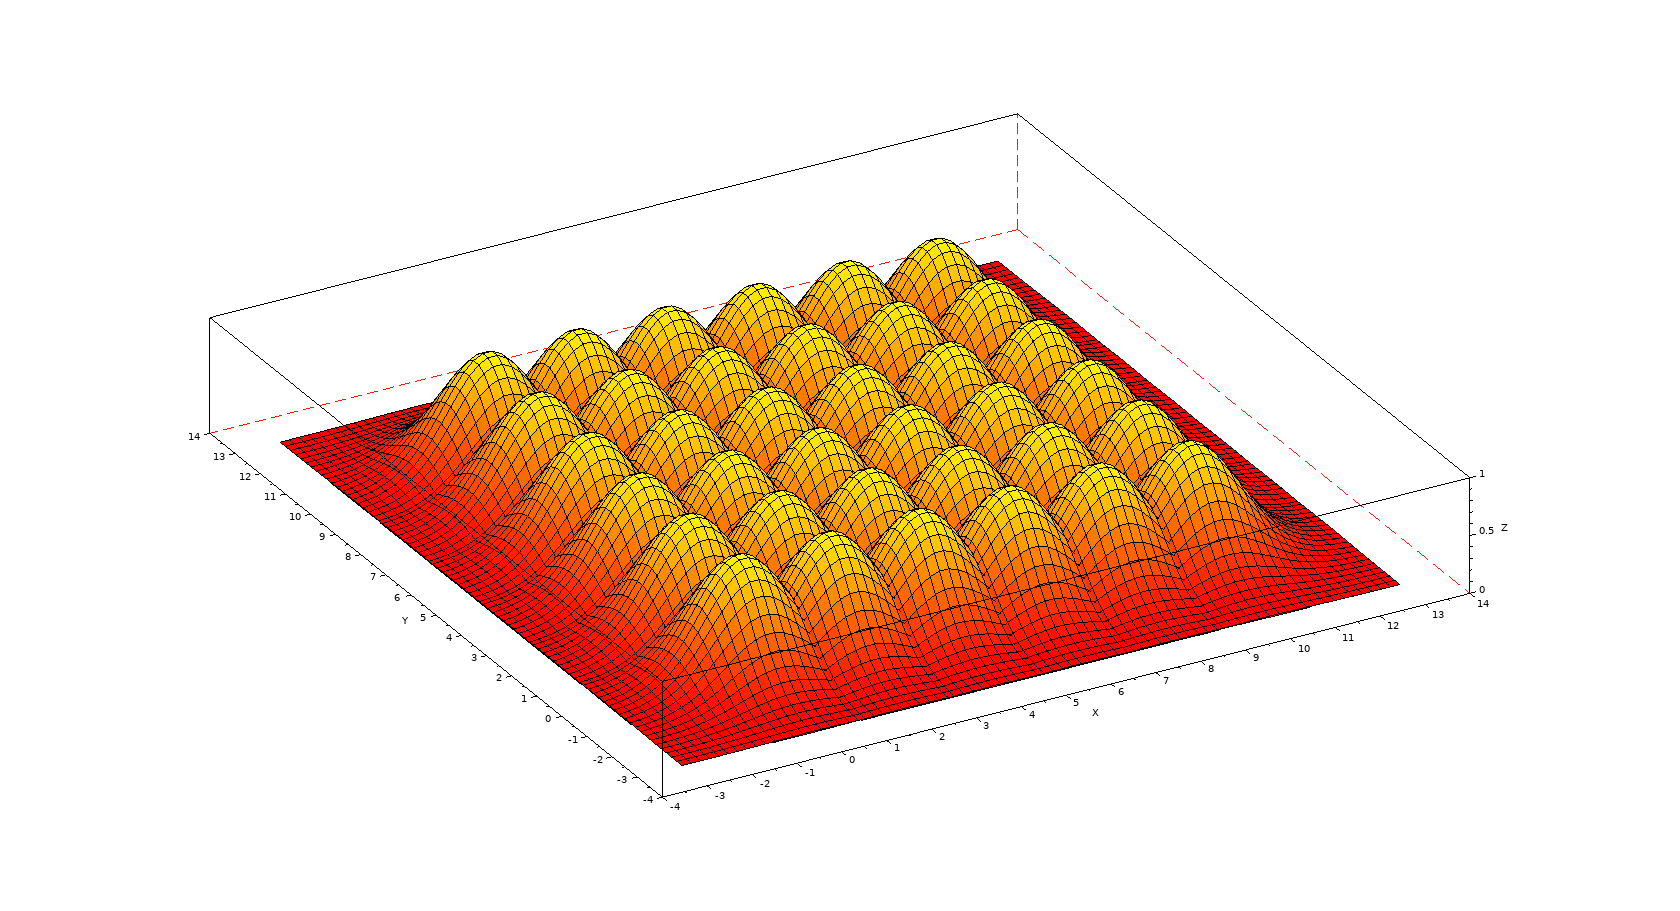
\includegraphics[scale=0.16]{matrixbubblesample.png}
\caption{Visual Representation of a Bubbled Grid\cite{bubble}}
\end{center}
\end{figure}

Once we've summarized both matrices $M$ and $N$ to $M'$ and $N'$ with lower
dimensions, we can now proceed to compare. As a result of the nature of our
reduction (with probability distributions), we cannot simply use any of the
regular distance metrics like euclidean, Lp norm, etc. This is because we could
have two normal distributions that are the same but orders of magnitude away
from each other by euclidean distance, etc so we need a theoretical sound way
of comparing probability distributions.

\section{Methods}

For our data set, we started with a set of black cursive letters.

\begin{figure}[h!]
\begin{center}

\includegraphics[scale=0.16]{alphabet_cursive_letter_a.jpg}
\caption{Sample Cursive Letter}
\end{center}
\end{figure}

We then tried to apply some morphological operators to the letter `a' to
perturb the image. This was so that we could compare this image with the
original image and see whether the scores indicated that the images were
similar. We also compared them to different letters to see if the scores
indicated the images were different.

\subsubsection{Morphological Operators}

Morphological operations apply a structuring element to an input image,
creating an output image of the same size. In a morphological operation, the
value of each pixel in the output image is based on a comparison of the
corresponding pixel in the input image with its neighbors. By choosing the size
and shape of the neighborhood, you can construct a morphological operation that
is sensitive to specific shapes in the input image.\cite{morph}\\

We'll use the following morphological operations to try to mimic real life
transformations to images. A lot of work is currently being done in the area of
interpreting historical maps. Historical maps help us understand how
geographical locations change. Because of how old some historical maps are,
they may have undergone various transformations. Dilation and erosion are some
morphological operations that are able to mimic these historical
transformations.

\subsubsection{Dilation and Erosion}

Dilation and erosion are two examples of morphological operations. Dilation
adds pixels to the boundaries of objects in an image, while erosion removes
pixels on object boundaries. The number of pixels added or removed from the
objects in an image depends on the size and shape of the structuring element
used to process the image. In the morphological dilation and erosion
operations, the state of any given pixel in the output image is determined by
applying a rule to the corresponding pixel and its neighbors in the input
image. The rule used to process the pixels defines the operation as a dilation
or an erosion. \cite{dilation}

\begin{figure}[h]
\centering
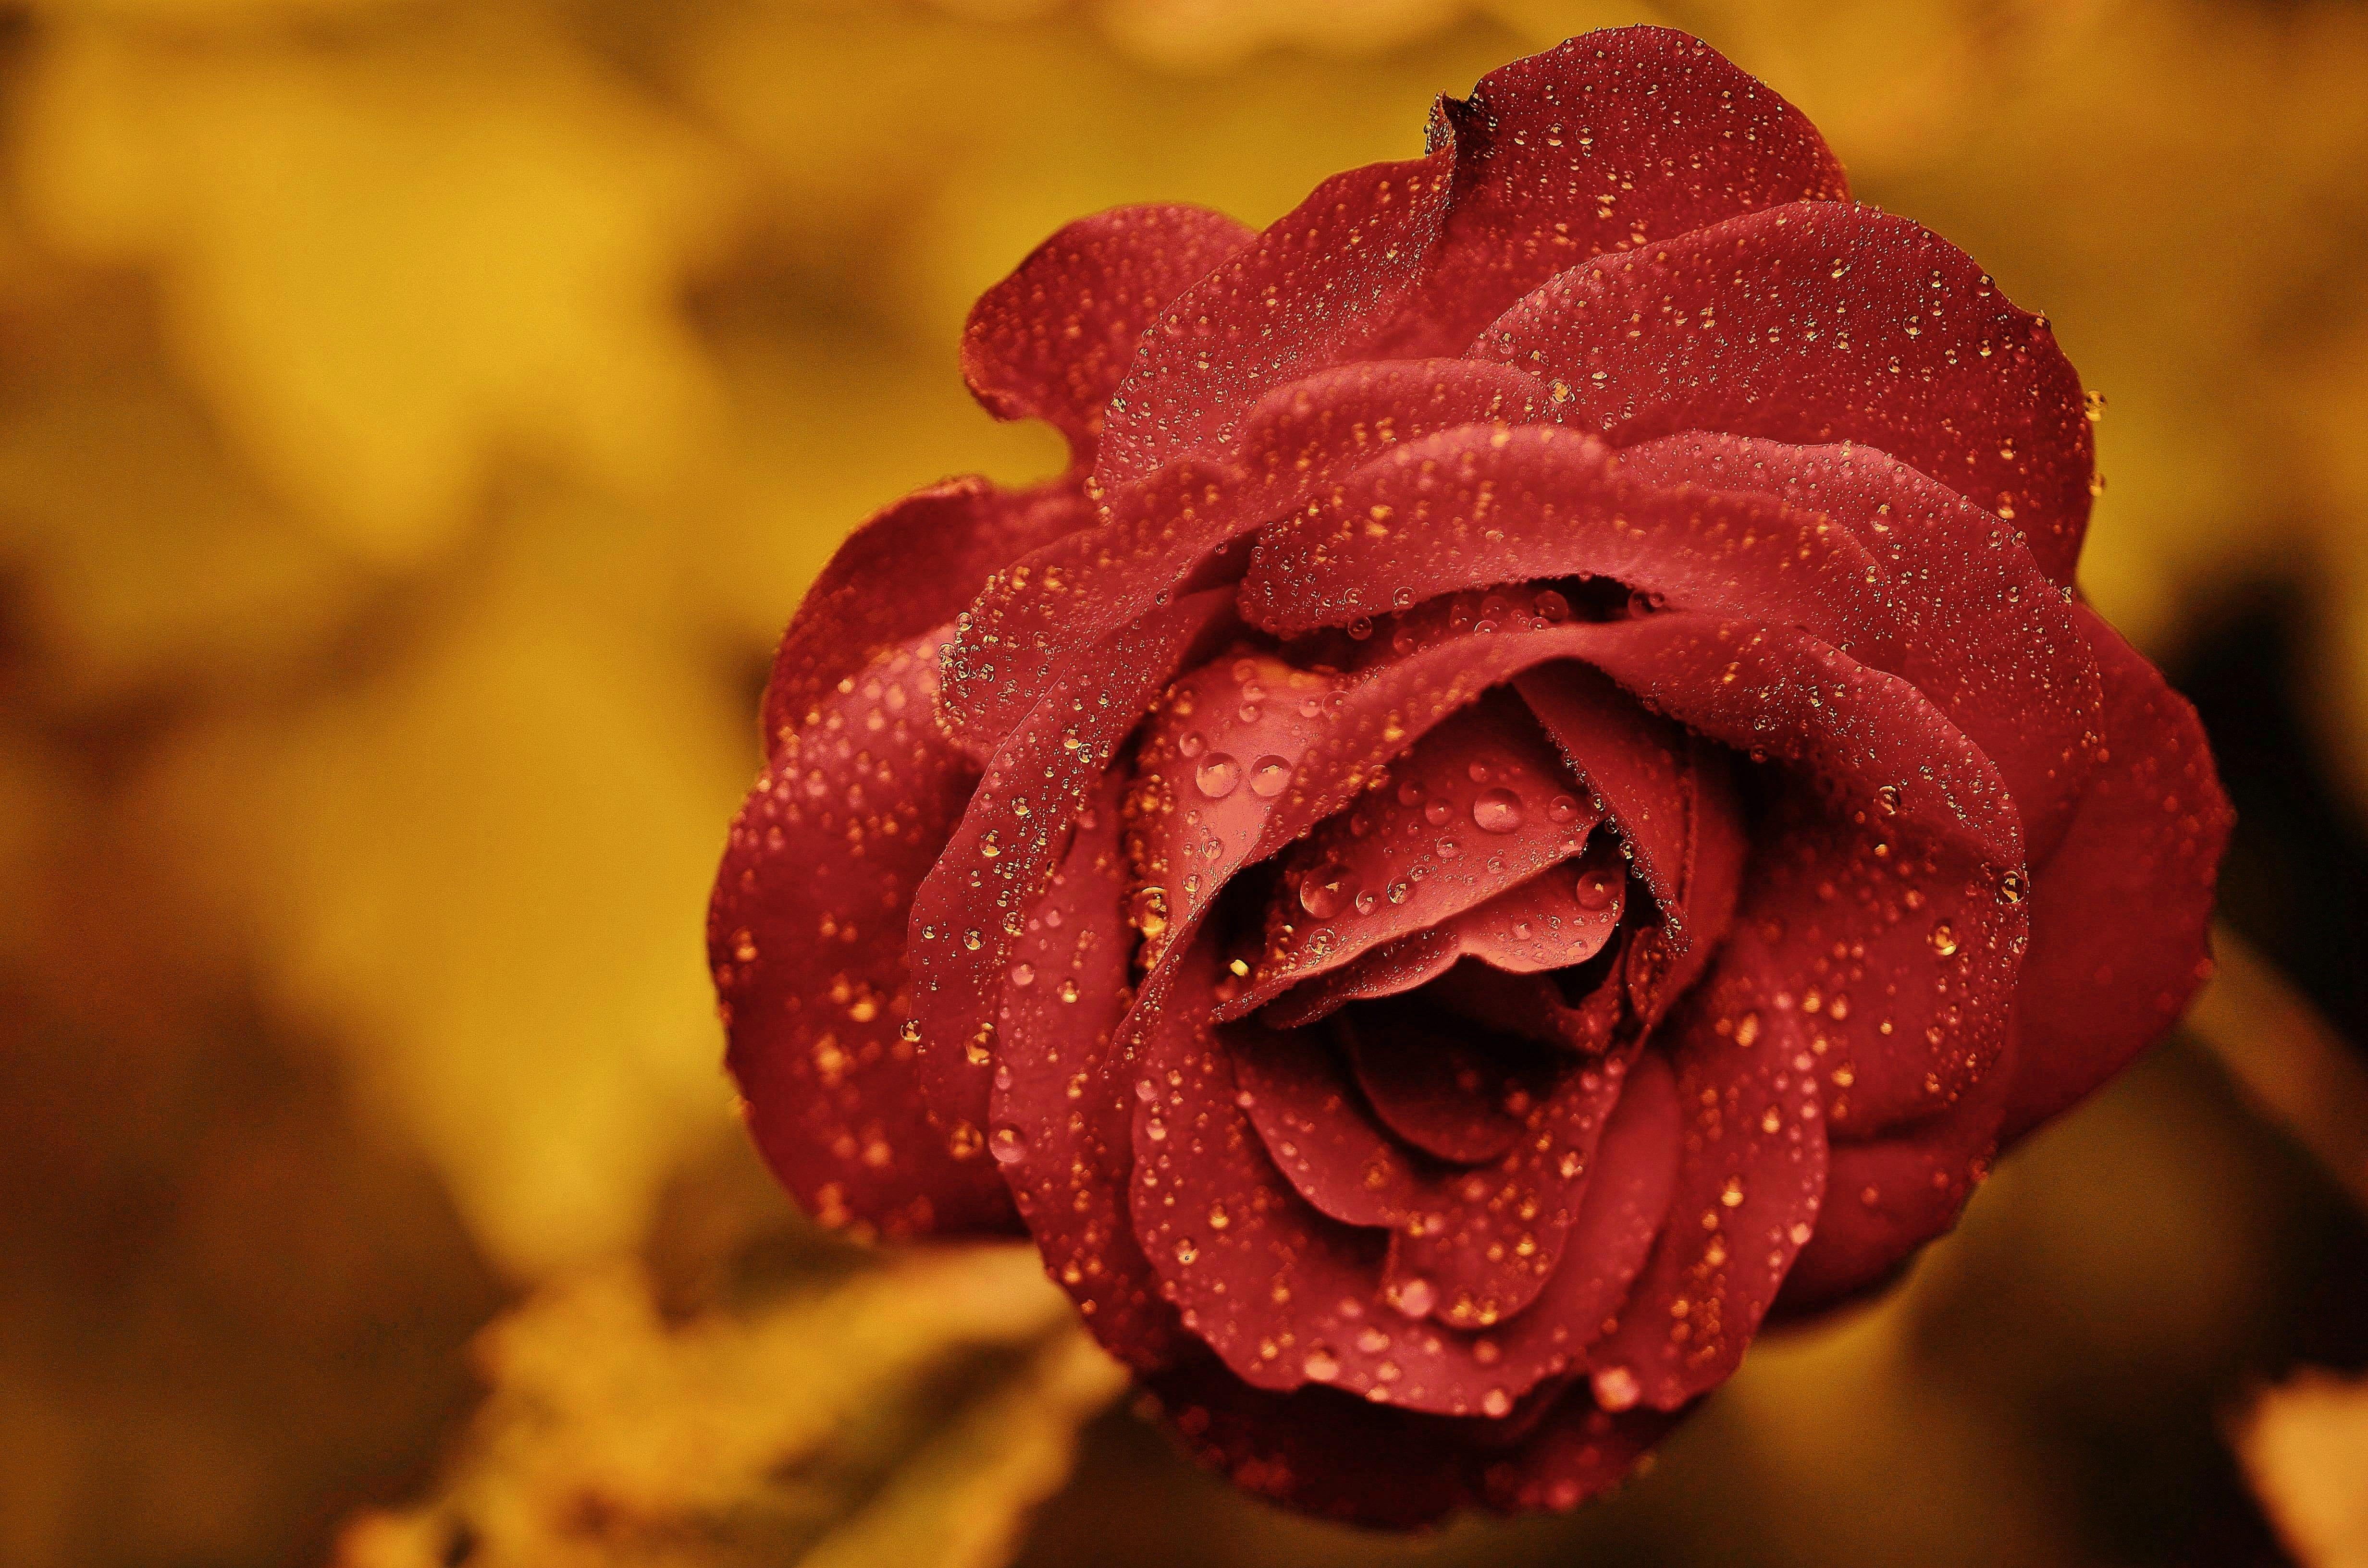
\includegraphics[scale=0.05]{cv_flower.jpg}
\caption{Flower Sample}
\end{figure}

Dilation - The value of the output pixel is the maximum value of all the pixels
in the input pixel's neighborhood. In a binary image, if any of the pixels is
set to the value 1, the output pixel is set to 1. See figure 4.

\begin{figure}[h!]
\centering
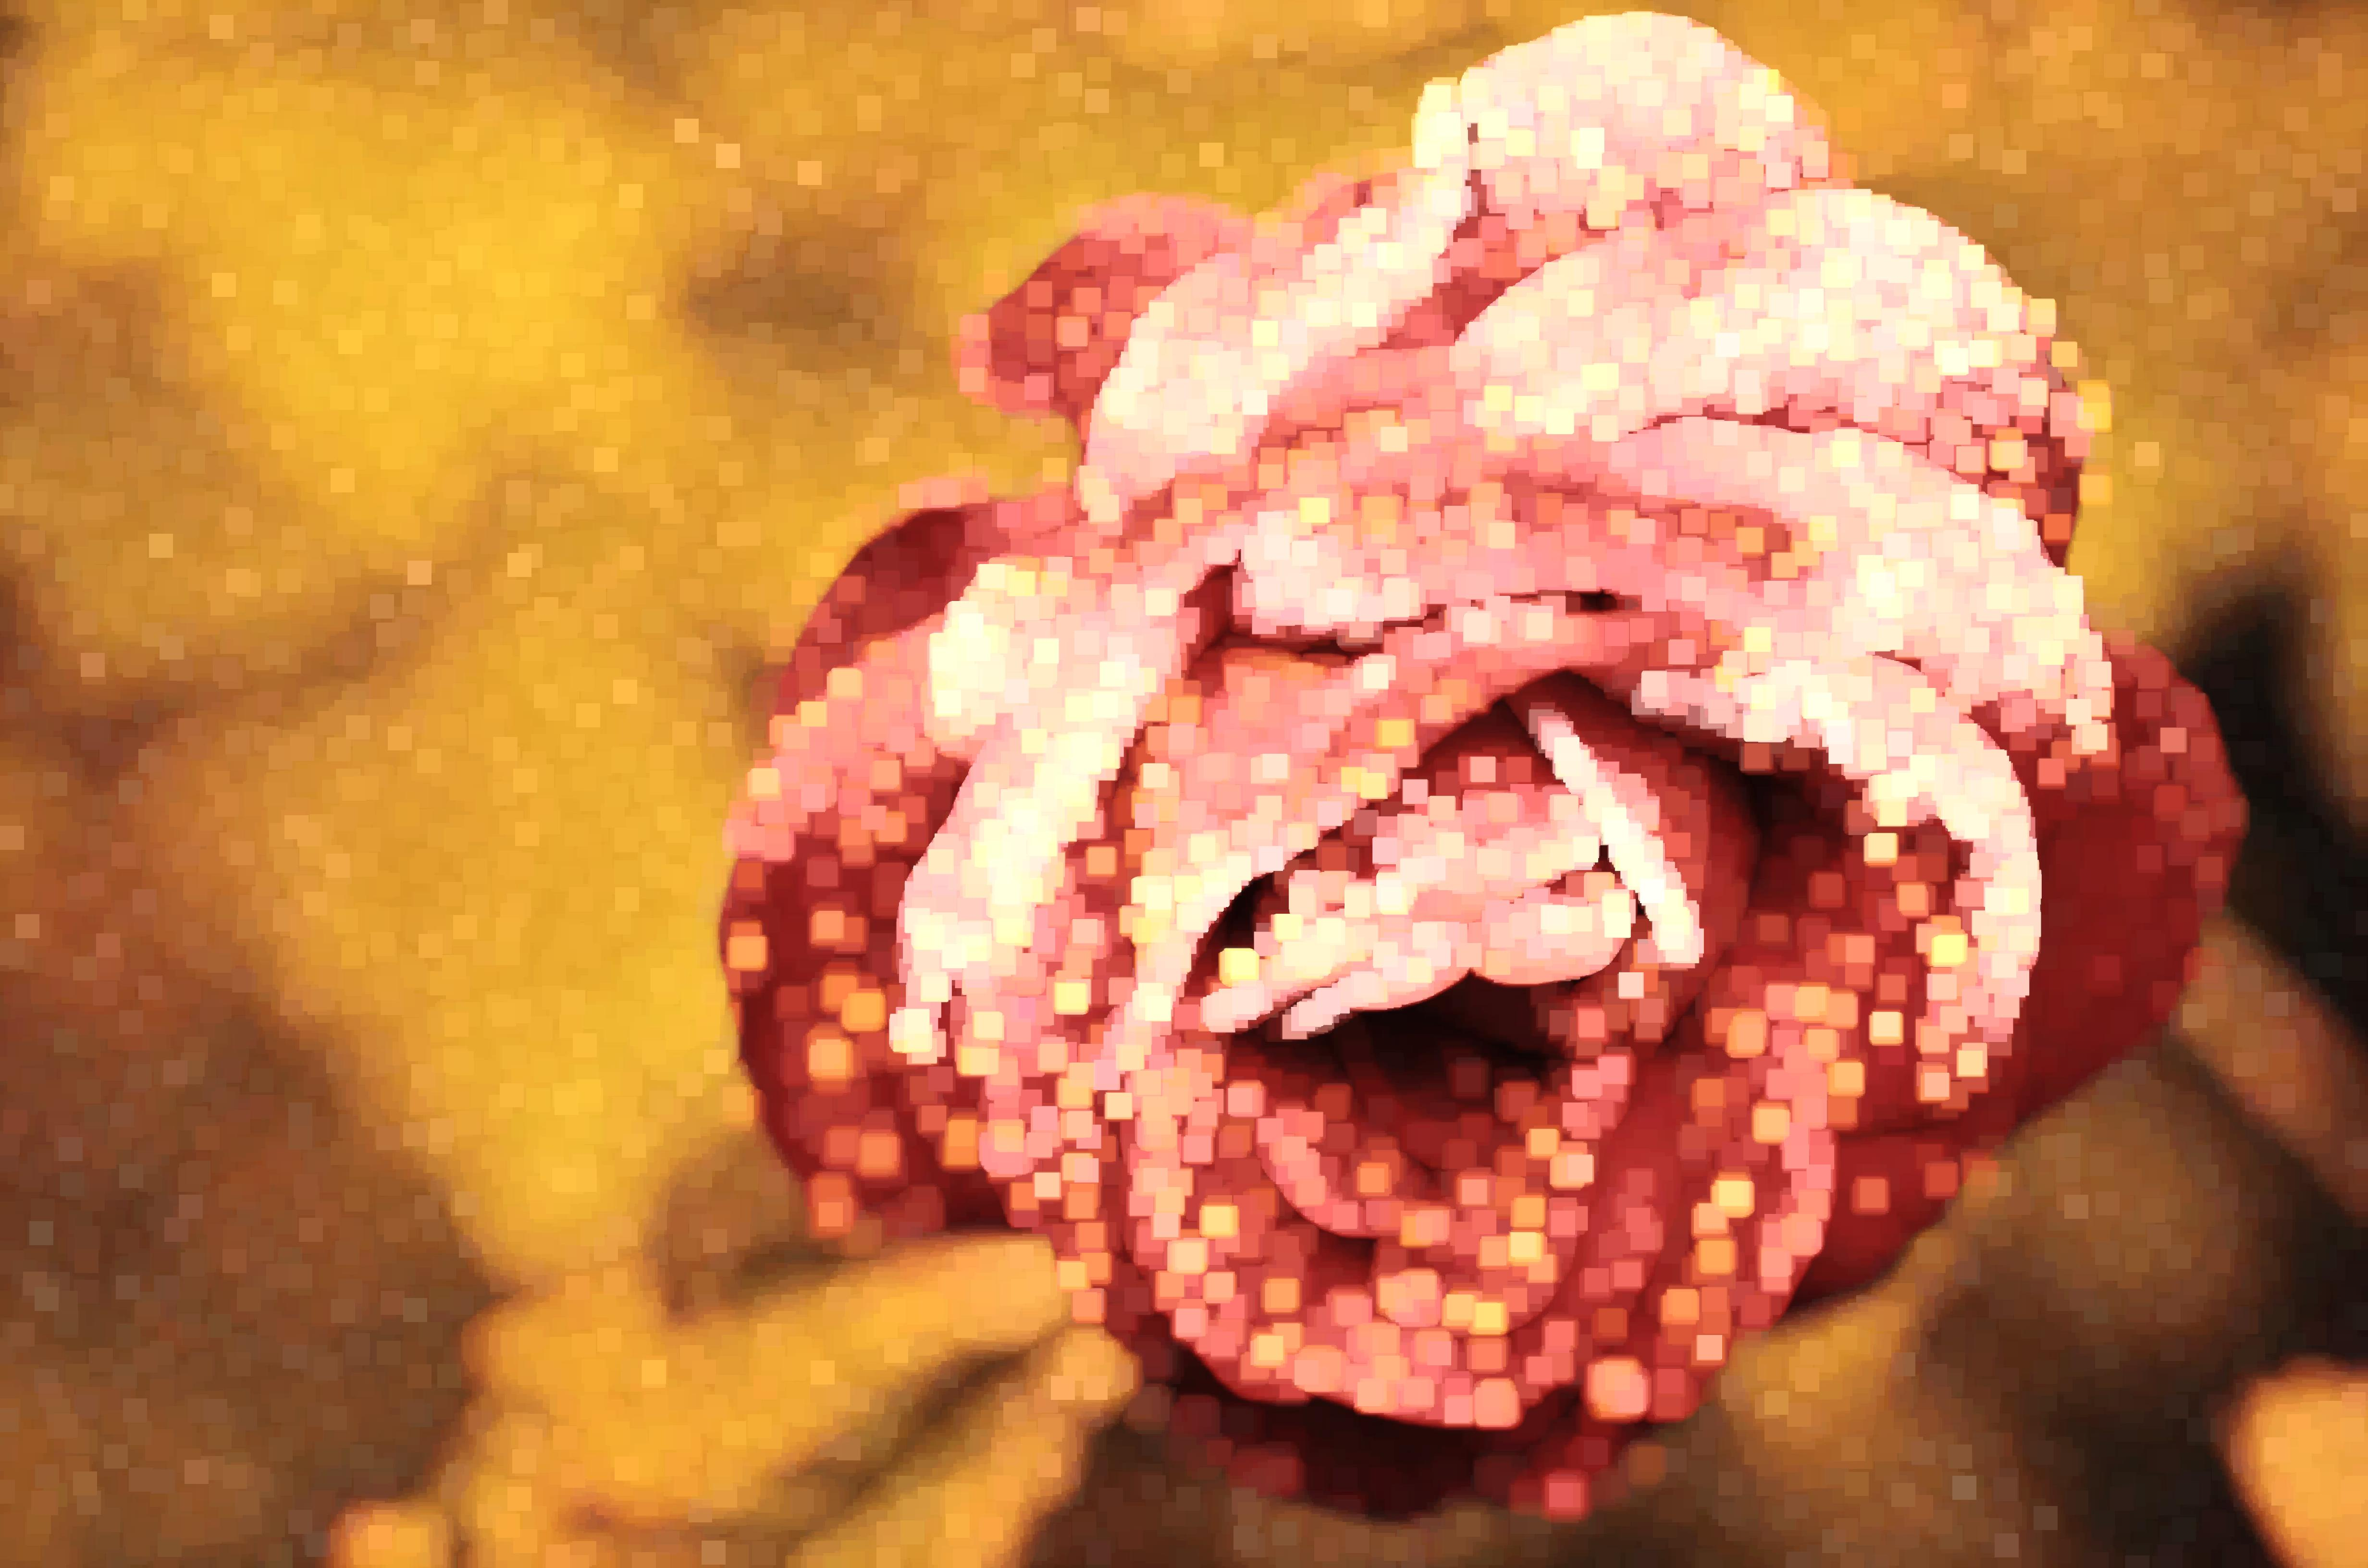
\includegraphics[scale=0.05]{dilated_flower.jpg}
\caption{Dilated flower}
\end{figure}

Erosion - The value of the output pixel is the minimum value of all the pixels
in the input pixel's neighborhood. In a binary image, if any of the pixels is
set to 0, the output pixel is set to 0. See figure 5.

\begin{figure}[h!]
\centering
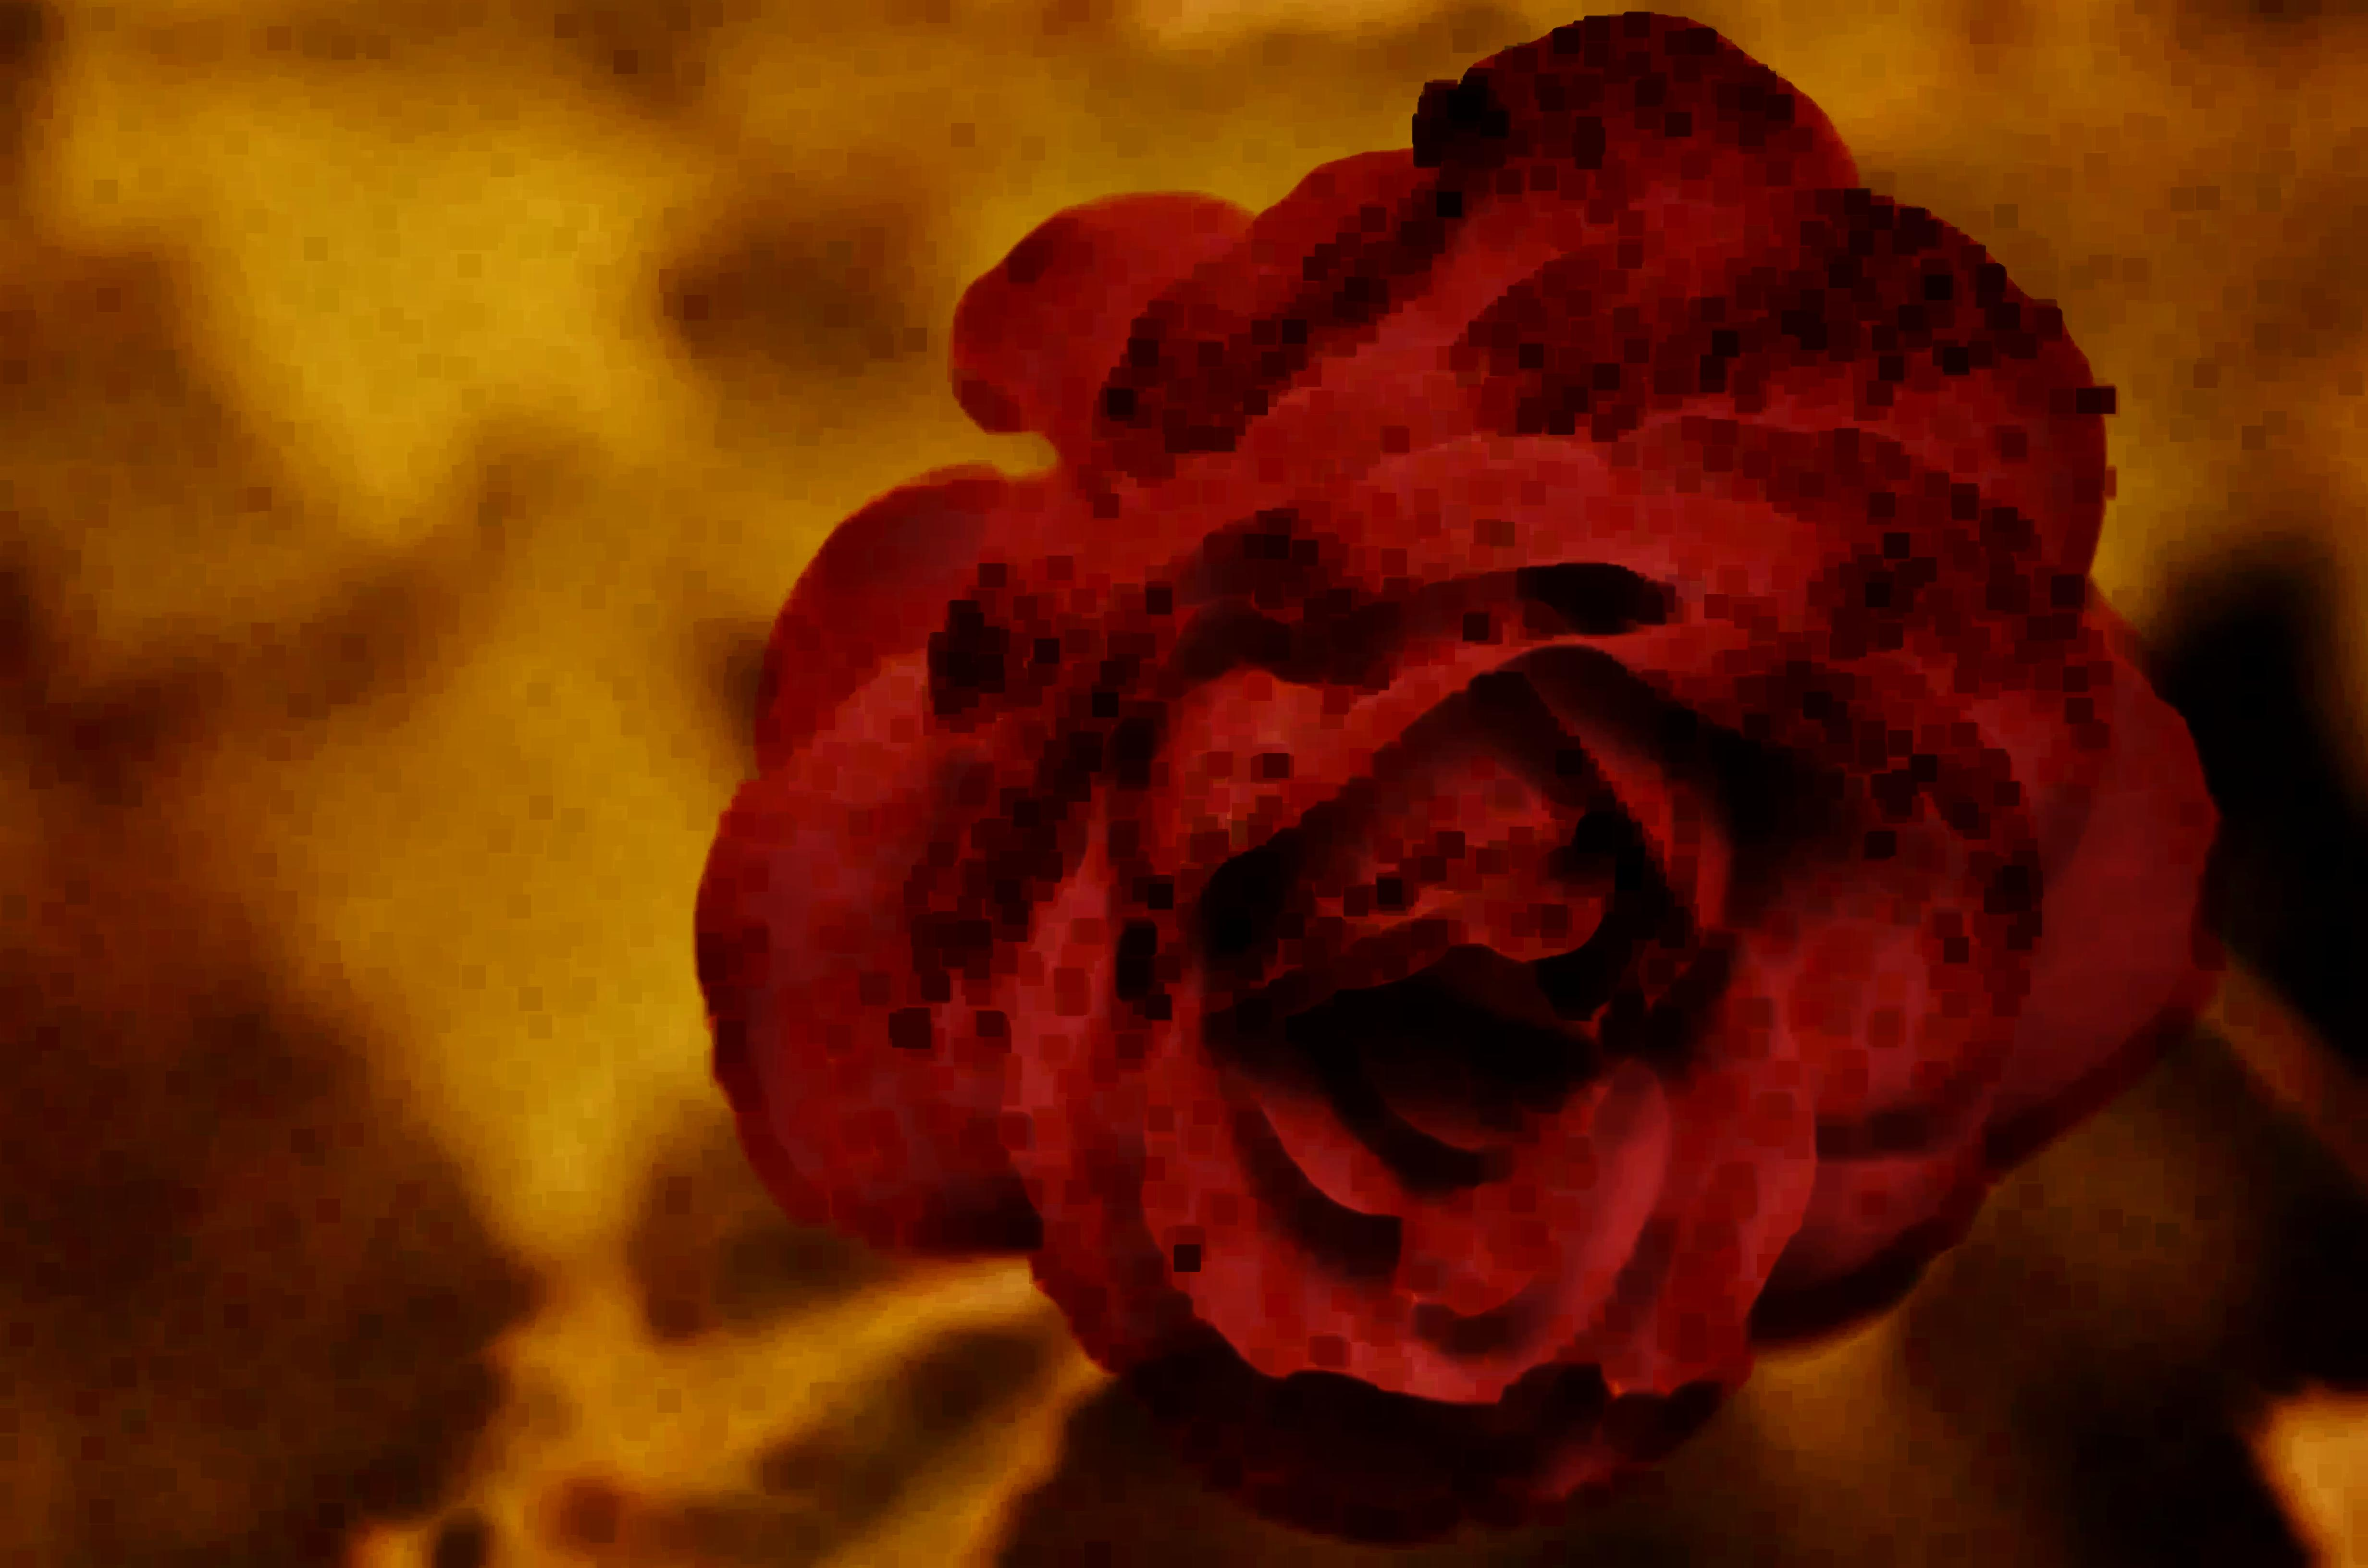
\includegraphics[scale=0.05]{eroded_flower.jpg}
\caption{Eroded flower}
\end{figure}

\subsection{Adding Random Noise}

Adding random noise to an image involves first generating an image of same size
as the original image with pixel values from a random distribution. In our
case, we choose to use the normal distribution. Then we add the generated image
to the original image (which one can think of as an overlay). See figure 6
below.

\begin{figure}[h!]
\centering
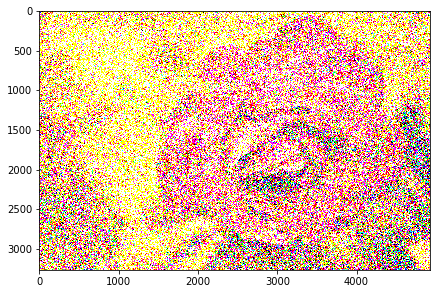
\includegraphics[scale=0.6]{noisy_flower.png}
\caption{Noisy flower}
\end{figure}

\subsection{Bubble Analysis}

Given two matrix bubblings of two images,we need a way to find the distance
between them. This is accomplished by finding the distance between each bubble,
and then combining the distance of all the bubbles. The distance between two
bubbles can be found using a variety of statistical distances, summarized in
the next section. Once we have a distance $d$ that computes the distance
between two bubbles, the total distance between the matrices is given as the
$L^1$ norm of the bubble distances. If $P_{ij}$ are the bubbles of the first
matrix and $Q_{ij}$ are the bubbles of the second, then the total distance is
given by
\[
    \sum_{i,j} d(P_{ij},Q_{ij}).
\]
It is possible that some bubbles would not have any data in them, which could
be because the data is missing or otherwise does not exist in that area. In
that case, there is no distribution for that bubble, so it is not included in
the sum to calculate the total distance.

\subsection{Distance Metrics}

For comparing two bubbles, we considered several distance metrics.

\subsubsection{Bhattacharyya Distance}

The Bhattacharyya distance is a measure of distance between probability
distributions related to the Hellinger distance. Like the Hellinger distance,
it is a metric, satisfying the triangle inequality. The Bhattacharyya distance
between two probability distributions $P$ and $Q$ with distribution functions
$p(x)$ and $q(x)$ is given by \cite{pardo}
\[
    B(P,Q)=-\log\int\sqrt{p(x)q(x)}\,dx.
\]
This is similar to the Hellinger distance, which is
\[
    H(P,Q)=\Pn{1-\int\sqrt{p(x)q(x)}\,dx}^{1/2}.
\]
The relationship between the two of them is given by
\[
    B(P,Q)=-\log(1-H^2(P,Q)).
\]
For a multivariate normal distribution, we can use the value of $H(P,Q)$ given
above to derive
\begin{multline*}
    B(P,Q)=-\log\frac{\det\Sigma_1^{1/4}\det\Sigma_2^{1/4}}
    {\det\Pn{\frac{\Sigma_1+\Sigma_2}{2}}^{1/2}}\\
    +\frac18(\mu_1-\mu_2)^T\Pn{\frac{\Sigma_1+\Sigma_2}{2}}^{-1}
    (\mu_1-\mu_2).
\end{multline*}
Note that if $B$ and $H$ are small, then to first order we have $B(P,Q)\approx
H^2(P,Q)$.

\subsubsection{Hellinger Distance}

The Hellinger distance is another measure of the distance from one probability
distribution to another. It is a metric, meaning that it is symmetric in its
arguments and satisfies the triangle inequality. The Hellinger distance between
two probability distributions is given by
\[
    H^2(P,Q)=1-\int \sqrt{f(x)g(x)}\,dx.
\]
For multivariate normal distributions $P$ and $Q$, where $P$ has mean $\mu_1$
and covariance matrix $\Sigma_1$ and $Q$ has mean $\mu_1$ and covariance matrix
$\Sigma_2$, the Hellinger distance is given by \cite{pardo}
\begin{multline*}
    H^2(P,Q)=1-\frac{\det\Sigma_1^{1/4}\det\Sigma_2^{1/4}}
    {\det\Pn{\frac{\Sigma_1+\Sigma_2}{2}}^{1/2}}\\
    \exp{-\frac18(\mu_1-\mu_2)^T\Pn{\frac{\Sigma_1+\Sigma_2}{2}}^{-1}
    (\mu_1-\mu_2)}
\end{multline*}

\subsubsection{KL Divergence}

The KL divergence is a measure of the distance from one probability
distribution to another. Given a probability distribution $P$ and another
distribution $Q$, the KL divergence from $P$ to $Q$ can be thought of as a
measure of how well the distribution $Q$ approximates $P$. It is defined by
\[
    D_{KL}(P\| Q)=\int_{-\infty}^\infty p(x)\log\Pn{\frac{p(x)}{q(x)}}\,dx,
\]
where $p(x)$ and $q(x)$ are the probability density functions of $p$ and $q$.
Since this distance is not symmetric in $P$ and $Q$, it is not a true metric.
Instead, we can use the \emph{symmetrized KL divergence}, defined by
\[
    D_{KLs}(P,Q)=\frac12 (D_{KL}(P\| Q)+D_{KL}(Q\| P)).
\]
Since we are approximating the data using normal distributions, we need a
formula for the KL divergence from one normal distribution to another. Let $P$
be a distribution with mean $\mu_1$ and covariance matrix $\Sigma_1$, and $Q$ a
distribution with mean $\mu_2$ and covariance matrix $\Sigma_2$. Then the
probability density functions for $P$ and $Q$ are
\begin{align*}
    p(x) &= \frac{1}{\sqrt{(2\pi)^n\det\Sigma_1}}e^{-\frac12(x-\mu_1)^T \Sigma_1^{-1}(x-\mu_1)}\\
    q(x) &= \frac{1}{\sqrt{(2\pi)^n\det\Sigma_2}}e^{-\frac12(x-\mu_2)^T \Sigma_2^{-1}(x-\mu_2)}\\
\end{align*}
and the $\log(p(x)/q(x))$ is given by
\begin{multline*}
    \log\Pn{\frac{p(x)}{q(x)}}=\\ \frac12\log\frac{\det\Sigma_2}{\det\Sigma_1} +\frac12(x-\mu_2)^T\Sigma_2^{-1}(x-\mu_2)-\frac12(x-\mu_1)^T \Sigma_1^{-1}(x-\mu_1).
\end{multline*}
The quantity that we are looking for is the integral of $p(x)\log(p(x)/q(x))$.
To make it easier to integrate, we can shift $x$ by $\mu_1$ and let
$\Delta\mu=\mu_2-\mu_1$ to get
\begin{multline*}
    p(x)\log\frac{p(x)}{q(x)}=\frac{1}{2\sqrt{(2\pi)^n\det\Sigma_1}}\\
    \Pn{\log\frac{\det\Sigma_2}{\det\Sigma_1}+(x-\Delta\mu)^T\Sigma_2^{-1}(x-\Delta\mu)-x^T\Sigma_1^{-1}x}e^{-\frac12x^T\Sigma_1^{-1}x}
\end{multline*}
Since any term with a single $x$ is odd and goes to zero in the integral, the
KL divergence is equal to
\[
    D_{KL}(P\| Q)=\frac{1}{2\sqrt{(2\pi)^n\det\Sigma_1}} \int (C+x^T(\Sigma_2^{-1}-\Sigma_1^{-1})x)e^{-\frac12 x^T\Sigma_1^{-1}x}\,d^nx,
\]
where
\[
    C=\log\frac{\det\Sigma_2}{\det\Sigma_1}+\Delta\mu^T\Sigma_2^{-1}\Delta\mu
\]
To evaluate the integral, we need to make use of the Gaussian integral
\[
    \int e^{-\frac12 x^TAx}\,d^nx=\sqrt{\frac{(2\pi)^n}{\det A}},
\]
for a symmetric matrix $A$, as well as the the following integral (see
\cite{zee}, pages 14-16):
\[
    \int x_ix_je^{-\frac12 x^TAx}\,d^nx=(A^{-1})_{ij}\sqrt{\frac{(2\pi)^n}{\det A}}
\]
Given another symmetric matrix $B$, we can take linear combinations of the
above integral to derive
\[
    \int x^TBx\,e^{-\frac12 x^TAx}\,d^nx=\sqrt{\frac{(2\pi)^n}{\det A}}\Tr{A^{-1}B}
\]
Using these two integrals, we can calculate the KL divergence to be
\begin{align*}
    D_{KL}(P\| Q)&=\frac12 C+\frac12\Tr(\Sigma_1(\Sigma_2^{-1}-\Sigma_1^{-1}))
    =\frac12 C-\frac n2+\frac12\Tr(\Sigma_1\Sigma_2^{-1})\\
    &=\frac12\Pn{\log\frac{\det\Sigma_2}{\det\Sigma_1}+\Delta\mu^T\Sigma_2^{-1}\Delta\mu+\Tr(\Sigma_1\Sigma_2^{-1})-n}
\end{align*}

\subsubsection{Fisher Information}

One way that the KL divergence can be made symmetric is by symmetrizing it as
described above, to get the symmetric KL divergence. Another way to get a
metric from the KL divergence is to look at the Hessian with respect to $Q$ for
a fixed $P$. Doing so will give a matrix which can be interpreted as a
Riemannian metric tensor. This metric tensor can then be used to get a metric
on the manifold of probability distributions, and the metric is called the
Fisher information metric. If the probability distributions depend on some
variables $\theta_i$, then the KL divergence is
\[
    D_{KL}(P(\theta^0)\| P(\theta))=-\int p(x;\theta^0)\log\frac{p(x;\theta)}{p(x;\theta^0)}\,dx
\]
Taking the derivative of the integrand with respect to first $\theta_i$, we get
\[
    -p(\theta^0)\frac{1}{p(\theta)}\frac{dp}{d\theta_i}.
\]
(At this point, if we let $\theta=\theta_0$, when we integrate over all $x$ we
get $0$, as expected.) Then taking a second derivative with respect to
$\theta_j$ we get
\[
    p(\theta^0)\frac{1}{p(\theta)^2}\frac{dp}{d\theta_i}\frac{dp}{d\theta_j} -p(\theta^0)\frac{1}{p(\theta)}\frac{d^2p}{d\theta_id\theta_j}
\]
When we let $\theta=\theta_0$ and integrate over all $x$, the second term goes
to zero, and we are left with
\[
    \int \frac{1}{p(x;\theta)}\frac{dp}{d\theta_i}\frac{dp}{d\theta_j}\,dx.
\]
Using the fact that
\[
    \frac{d\log p(x;\theta)}{d\theta_i}=\frac{1}{p(x;\theta)}\frac{dp(x;\theta)}{d\theta_i},
\]
we can recover the more familiar form
\[
    \int \frac{d\log p(x;\theta)}{d\theta_i}\frac{d\log p(x;\theta)}{d\theta_j}p(x;\theta)\,dx.
\]
On the space of single-variate Gaussian distributions, there are only two
parameters, the mean $\mu$ and the variance $\sigma$. That means that the
metric tensor is a $2\times 2$ matrix, and it happens to equal
\[
    \frac{1}{\sigma^2}\begin{pmatrix}1&0\\0&2
    \end{pmatrix}.
\]
This is the same as the metric for the Poincare model of the hyperbolic plane,
so under the Fisher information metric, distances between two normal
distributions are the same as hyperbolic distances in the plane.\\

One potential future application of matrix bubbling that we have not yet
considered is to time series data. If the data is a continuous function of
time, then we would be interested in looking at the derivative. The Fisher
information metric can be of use in calculating this derivative. Given
$P(\theta)$ where the $\theta$ parameters are functions of the time variable
$t$, the derivative would be given by
\[
    \frac{d(P(\theta(t+\Delta t)),P(\theta(t)))}{\Delta t}
\]
Letting $\Delta\theta=\theta(t+\Delta t)-\theta(t)$, this is equal to
\[
    \frac{d(P(\theta+\Delta\theta),P(\theta))}{\Delta t}.
\]
The distance here could be any distance, but since the change in $\theta$ would
be small for a single time step, the Fisher information metric could be used as
a good approximation. If the metric tensor is $g_{ij}(\theta)$, then the
squared distance between $P(\theta+\Delta\theta)$ and $P(\theta)$ is
\[
    g_{ij}(\theta)\Delta\theta_i\Delta\theta_j.
\]
So the derivative is then equal to
\[
    \frac{\sqrt{g_{ij}(\theta)\Delta\theta_i\Delta\theta_j}}{\Delta t}
\]

\section{Results}

Below is a grid of images with morphological operators applied to them.

\begin{figure}[h!]
\begin{center}
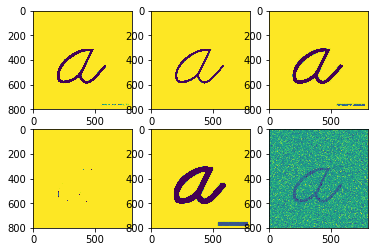
\includegraphics[scale=0.7]{a-grid.png}
\caption{Morphological Operators Applied on an Image}
\end{center}
\end{figure}

The first image is the original image. Sweeping from left to right then
downwards, we see that the second image (A) is an erosion, the third (B) is a
dilation, the fourth (C) is a stronger erosion, the fifth (D) is a stronger
dilation, and the sixth (E) has added random noise.\\

We compared each of the five morphed images with the original using both the
Hellinger distance and the KL divergence. The distances are recording in the
following table. Some of the comparisons did not work due to the code crashing
so we have put a `-' in the space to denote that we should ignore it for now.

\begin{figure}[h!]
\begin{center}
  \begin{tabular}{ c || c | c | c | c | c }
     & A & B & C & D & E \\ \hline
    Hellinger & -8.24 & 24.20 & 0.25 & 51.97 & - \\
    KL & 3092.31 & - & 3101.11 & - & -
  \end{tabular}
  \caption{Comparison of Morphed Letters with Original Letter}
\end{center}
\end{figure}

We also compared each of the five morphed images with the letter `B'. We did
this because we expect the distances to be greater since they are not the same
letter. The distances are recorded in the following table.

\begin{figure}[h!]
\begin{center}

\includegraphics[scale=0.16]{alphabet_cursive_letter_b.jpg}
\caption{Cursive Letter `B'}
\end{center}
\end{figure}

\begin{figure}[h!]
\begin{center}
  \begin{tabular}{ c || c | c | c | c | c }
     & A & B & C & D & E \\ \hline
    Hellinger & 14.72 & 45.15 & 1.26 & 54.18 & - \\
    KL & 35.55 & - & 330.40 & - & -
  \end{tabular}
  \caption{Comparison of Morphed Letters with Different Letter}
\end{center}
\end{figure}

For the Hellinger distance, we can see that the distances in figure 8 are
generally larger than those in figure 9. This makes sense since similar images
should give a smaller distance. For the same reason, the highly eroded image in
general had a larger distance compared to the other morphed images. We also see
that the scores for the strongly eroded images are lower than the others since
there are not much pixels to compare since we throw out grids with no pixels.
Also, we note that the first comparison gives us a negative number, which
should not be possible.\\

For the KL divergence, there seem to be much more errors and the trend seems to
be the opposite of what we expect. We see that similar images have high
divergence while different images have low divergence. This means that we
should probably not use the KL divergence.

% Values from previous analysis
% 14.378289414054253
% 175.12170883771097
% 115.76290575014204
% 54.12331211190002
% 141.55566167043116

\section{Future Work}

Our progress so far has been to understand and come up with an initial
implementation for the matrix bubbling technique. The next steps are to
investigate more applications of matrix bubbling, and specifically to see how
well it performs. We would also like to improve our code so it can run faster
and produce fewer errors.

\clearpage
\printbibliography

\end{document}
